\section{Algorithms}
\label{sec:Algorithm}
% In this section, we describe the details of our placement algorithm.
We will detail the placement algorithm in this section.

\iffalse
\begin{table}[tb]
   \centering
   \caption{The Architecture Notations}
   \resizebox{0.50\textwidth}{!}{
     \begin{tabular}{|ll|}
     \hline
     $S$ & The field type set \{LUTL, LUTM-AL, FF, CARRY, DSP, BRAM\}.\\
    %  $R$& The set of clock regions (CRs). \\
    %  $E$, $\mathcal{E}$ & The set of nets and the set of clock nets. \\
     $E$, $\mathcal{V}$ & The set of nets, and the instance set.\\
     $\mathcal{M}^s_i$ & The resource demand from field type $s \in S$ of instance $i \in \mathcal{V}$. \\
     $\mathcal{V}^r_s$ & The instance subset with resource demand from field type $s \in S$, namely $\{i \in \mathcal{V} \vert \mathcal{M}^s_i>0\}$. \\
    %  $\mathcal{V}^c_e$ & The instance subset whose elements are the clock sinks of clock net $e \in \mathcal{E}$. \\
    %  $\mathcal{A}^p$ & The physical instance areas. \\
    %  $w_e$ & The weight of net $e \in E$. \\
     %$\mathcal{L}_j$ & The subset of CRs that are left of or in the column above CR $j \in R$. \\
     %$\mathcal{R}_j$ & The subset of CRs that are right of or in the column above CR $j \in R$. \\
     %$\mathcal{U}_j$ & The subset of CRs that are above of or in the row above CR $j \in R$. \\
     %$\mathcal{D}_j$ & The subset of CRs that are bellow of or in the row above CR $j \in R$. \\
     \hline
     \end{tabular}
   }
   \label{tab:notations}
 \end{table}
% Among them, the detailed difference between notations LUTL and LUTM-AL will be introduced in \secRef{sec:clb_heter}.
\fi

\subsection{Overview of the Proposed Algorithm}
\label{sec:OverviewOfTheProposedFlow}

\begin{figure}[tb]
   \centering
   \includegraphics[width=\linewidth]{figs/overall_flow.pdf}
   \caption{The proposed Overall Flow.}
   \label{fig:overall_flow}
   \vspace{-.2in}
\end{figure}

% Our framework consists of two major phases:
% (1) nested global placement with timing awareness and clock feasibility,
% (2) clock-aware legalization and detailed placement, as shown in \figRef{fig:overall_flow}.
As illustrated in \figRef{fig:overall_flow}, our method includes two fundamental stages: (1)
nested global placement with timing awareness and clock feasibility, and (2)
clock-aware legalization and detailed placement.

\iffalse
We solve the clock-driven global placement problem using the Lagrangian relaxation multiplier method. In addition to the density constraint and density penalty, we also have the clock constraint as mentioned in \secRef{sec:clock_constraint}, with its penalty term and multiplier (hence referred to as clock penalty and clock multiplier). We also consider CARRY chain alignment constraints and routability constraints, which ensure better downstream performance in the legalization and routing phase.
\fi

% To handle SLICEL-SLICEM heterogeneity, we define the field type set as $S = $ \{LUTL, LUTM-AL, FF, CARRY, DSP, BRAM\} with special field setup (\secRef{sec:clb_heter}).
We cope with the SLICEL-SLICEM heterogeneity by defining the field type set as $S = $ \{LUTL, LUTM-AL, FF, CARRY, DSP, BRAM\} with a special field setup (\secRef{sec:clb_heter}).
% We formulate the problem as Formulation~(\ref{eq:opt_relax}), with clock constraints, carry chain alignment feasibility and timing optimization.
With clock constraints, carry chain alignment feasibility, and timing optimization, we formulate the problem as Formulation~(\ref{eq:opt_relax}).
 \begin{subequations}
   \label{eq:opt_relax}
  \begin{align}
    \min_{\boldsymbol{x}, \boldsymbol{y}} & \quad \widetilde{\mathcal{T}}_{\boldsymbol{\omega}}(\boldsymbol{x}, \boldsymbol{y}), \\
    \text{s.t.} & \quad \Phi_s(\boldsymbol{x}, \boldsymbol{y}; \mathcal{A}^s) = 0,\quad \forall s \in S, \\
    & \quad \varGamma(\boldsymbol{x}, \boldsymbol{y}) = 0, \\
    & \quad \text{\emph{Carry chain alignment constraint,}}
  \end{align}
\end{subequations}
%
$\widetilde{\mathcal{T}}_{\boldsymbol{\omega}}(\cdot)$ is the timing
performance objective,
%
where $\boldsymbol{\omega}$ measures the net criticality in the current timing graph
(\secRef{sec:timing_opt}).
%
$\mathcal{A}^s$ denotes the instance areas in the field $s$, 
%
and $\varGamma(\cdot)$ is the clock penalty term (\secRef{sec:cnp_algo}).
%
%We will discuss the definition of $\varGamma(\cdot)$ in detail in \secRef{sec:cnp_algo}.
For brevity, in later discussions, we condense $\Phi_s(\boldsymbol{x}, \boldsymbol{y};\mathcal{A}^s)$ to $\Phi_s$ for all $s \in S$,
and denote $\boldsymbol{\Phi}$ as the potential energy vector, whose components are the potential energy for each field, i.e., $\Phi_s(\forall s \in S)$.

% We leverage the \emph{augmented Lagrangian method (ALM)} \cite{andreani2008augmented} to formulate a better unconstrained subproblem,
We relax the original problem (\ref{eq:opt_relax}) by leveraging the \emph{augmented Lagrangian method (ALM)} \cite{andreani2008augmented} to formulate a better unconstrained subproblem,
%as shown in \eqRef{eq:opt_alm}:
\begin{subequations}
\begin{align}
  \min_{\boldsymbol{x}, \boldsymbol{y}} \quad \mathcal{L}(\boldsymbol{x}, \boldsymbol{y}; \boldsymbol{\lambda}, \boldsymbol{\mathcal{A}},\eta, \boldsymbol{\omega}) & =
   \widetilde{\mathcal{T}}_{\boldsymbol{\omega}}(\boldsymbol{x}, \boldsymbol{y})  + \sum\limits_{s \in S} \lambda_s \mathcal{D}_s \nonumber \\
   & + \eta \varGamma(\boldsymbol{x}, \boldsymbol{y}), \\
\mathcal{D}_s &= \Phi_s + \frac{1}{2}\mathcal{C}_s \Phi_s^2,\quad \forall s \in S,
\end{align}
\label{eq:opt_alm}
\end{subequations}
The density multiplier vector is $\boldsymbol{\lambda} \in \mathbb{R}^{\vert S \vert}$,
and the clock penalty multiplier is $\eta \in \mathbb{R}$.
The purpose of the weighting coefficient vector $\boldsymbol{\mathcal{C}} \in \mathbb{R}^{\vert S \vert}$ is to achieve a balance between the first-order and second-order terms for density penalty.
We follow the setup for $\boldsymbol{\lambda}$ and $\boldsymbol{\mathcal{C}}$ as \cite{PLACE_TCAD2021_Meng}.
% We also use $\mathcal{D}$ to denote $\boldsymbol{\Phi} + \frac{1}{2}\boldsymbol{\mathcal{C}} \odot \boldsymbol{\Phi}^2$ and omit $y$ for brevity.
% As we have multiple constraints, we leverage Lagrangian relaxation and break the problem into nested optimization problems,
To cope with multiple constraints, we rewrite the problem in a nested manner through the Lagrangian relaxation method,
\begin{subequations}
  \begin{align}
    \textrm{Timing Opt.: } \quad \mathcal{L}_1 & = \max_{\boldsymbol{\omega}} \mathcal{L}_2 (\boldsymbol{\omega}),  \\
    \textrm{Clock Opt.: } \quad \mathcal{L}_2(\boldsymbol{\omega}) & = \max_{\eta} \mathcal{L}_3 (\eta, \boldsymbol{\omega}), \\
    \textrm{Routability Opt.: } \quad \mathcal{L}_3(\eta, \boldsymbol{\omega}) & = \max_{\boldsymbol{\mathcal{A}}} \mathcal{L}_4 (\boldsymbol{\mathcal{A}}, \eta, \boldsymbol{\omega}),  \\
    \textrm{Wirelength Opt.: } \quad \mathcal{L}_4(\boldsymbol{\mathcal{A}}, \eta, \boldsymbol{\omega}) & = \max_{\boldsymbol{\lambda}} \mathcal{L}_5 ( \boldsymbol{\lambda},  \boldsymbol{\mathcal{A}}, \eta, \boldsymbol{\omega}),\label{eq:nested_opt_density} \\
    \textrm{Subproblem: } \quad \mathcal{L}_5(\boldsymbol{\lambda}, \boldsymbol{\mathcal{A}}, \eta, \boldsymbol{\omega}) & = \min_{\boldsymbol{x}, \boldsymbol{y}} \mathcal{L}(\boldsymbol{x}, \boldsymbol{y}; \boldsymbol{\lambda}, \boldsymbol{\mathcal{A}},\eta, \boldsymbol{\omega}),
  \end{align}
  \label{eq:nested_opt}
\end{subequations}
where $\mathcal{L}_5$ denotes \eqRef{eq:opt_alm}.
% Each problem passes its variables to the subproblem as fixed hyperparameters.
To put it simply, a set of variables in the objective function is constrained to be the optimal solution of the extra optimization problem,
and the variables of the exterior optimization problem are passed toward the sub-problem as fixed parameters.
To illustrate, take the solving process of $\mathcal{L}_5$ as an example.
The subproblem $\mathcal{L}_5$ aims at finding the optimal instance positions $\boldsymbol{x}$ and $\boldsymbol{y}$
given a set of fixed parameters $\boldsymbol{\lambda}$, $\boldsymbol{\mathcal{A}}$, $\eta$, and $\boldsymbol{\omega}$ from $\mathcal{L}_4$.
When $\mathcal{L}_5$ comes to the convergence to its minimum solution,
the $\mathcal{L}_4$ optimizer will improve the parameter $\boldsymbol{\lambda}$
so as to enlarge the magnitude of the density terms in the overall optimization objectives.
Therefore, the $\mathcal{L}_5$ optimizer will try to find a better solution by moving the instances to a less dense region in a new iteration,
and thus the density constraints will be forced to be gradually adequate.
We also adopt the same procedure to solve the other subproblems.
%To consider multiple constraints, the optimization is performed in nested loops of iterations, as shown in \figRef{fig:overall_flow}. The innermost loop is the diverge-aware Nesterov optimization, where we seek to solve the unconstrained problem in \eqRef{eq:opt_alm} given fixed density and clock multipliers.
%%We refer each optimization step of this problem as one \emph{iteration}.
%Everytime the innermost problem converges, we increase the density multiplier.
%After some iterations, when the density constraints are considered satisfied, we then go to the outer loop, to adjust the routability constraints' "multiplier". When both constraints are satisfied, we then go to the outmost loop and activate the clock contraints. When all three constraints are satisfied, and the wirelength changes very little between two iterations, we call it a close for global placement, and preceed onto the legalization phase.
%The density constraints are considered satisfied when \emph{overflow}, i.e. the fraction between the overlapped area between the instances and the area of all instances, for all fields are small enough.

\figRef{fig:overall_flow} depicts the nested loops to solve the problem.
$\mathcal{L}_1$ aims at improving the timing slacks via the timing-criticality-based weighting method.
The stopping criterion of $\mathcal{L}_1$ is whether timing slacks can be improved (\secRef{sec:timing_opt}).
$\mathcal{L}_2$ (\secRef{sec:cnp_algo}) aims at excluding the cases where clock routing is illegal under an analytical formulation.
We regard $\mathcal{L}_2$ as converged when there is no clock violation (\secRef{sec:clock_constraint}).
% The stopping criteria of $\mathcal{L}_2$ is whether the clock constraints are satisfied (\secRef{sec:clock_constraint}).
$\mathcal{L}_3$ develops the area inflation-based technique from \cite{PLACE_TCAD2021_Meng} in order to optimize the routability,
and the estimated routing congestion and pin density are the convergence criteria of $\mathcal{L}_3$.
% the stopping criteria of $\mathcal{L}_3$ is determined by routing congestion estimation and pin density.
$\mathcal{L}_4$ is the core wirelength-driven placement problem.
We empirically find that the density \emph{overflow} is a good indicator of the density constraints.
% The stopping criteria for $\mathcal{L}_4$ is determined by the density \emph{overflow} of all.
\footnote{
  We set the overflow threshold for LUTs and FFs to 10\% in our experiments.
}
For $\mathcal{L}_5$, we always solve with a fixed number of iterations, e.g., one iteration in the experiments.

\iffalse
The stopping criteria of $\mathcal{L}_3$ is determined by routing congestion estimation and pin
density, as $\mathcal{L}_3$ optimizes the routability essentially by instance area inflation
\cite{PLACE_TCAD2021_Meng}.
\fi
\iffalse
When the inner sub-problem $\mathcal{L}_3$ converges, we inflate the instances' area according to their location's routing congestion estimation.
Analogically, instances in routing congested areas will have more amount of charges in the electrostatic system (see \figRef{fig:electrostatics_analogy}) and are thus being spread out from the routing congested areas.
\fi

%The clock constraints are considered satisfied when the placement is compatible with the target architecture in \secRef{sec:clock_constraint}.

%As discussed in \secRef{sec:multi_electrostatics_placement}, the routability constraints does not have a term in the objective \textit{per se}, nor does it have a "multiplier".
%Rather, the "multiplier" function is achieved by inflating the instance areas, so the routability of the design is represented in the density constraint term\cite{PLACE_TCAD2021_Meng}. Downstream routing congestion, pin density and downstream clustering compatibility are all considered. The satisfaction of routability constraints is based on heuristics involving the overflow of LUTs and FFs.
%\footnote{
%  In our experiments, the target is empirically set to 10\% overflow for LUTs and FFs.
%}

In each iteration, we resolve the carry chain alignment constraints through
iterative support from \emph{iterative carry chain alignment correction}
(\secRef{sec:carry_alignment}).
% The carry chain alignment constraint is resolved through \emph{iterative
% carry chain alignment correction} in each iteration
% (\secRef{sec:carry_alignment}).
Following placement, we evolve clock-aware direct legalization and detailed placement algorithms that above clock feasibility constraints are met \cite{PLACE_TCAD2019_Li_UTPLACEF_DL}.
% After the placement phase, we develop clock-aware direct legalization and detailed placement algorithms based on
% \cite{PLACE_TCAD2019_Li_UTPLACEF_DL} to honor the aforementioned clock feasibility and SLICEL-SLICEM heterogeneity.
% Due to page limit, we omit the details on routability optimization, clock-aware legalization and detailed placement.
We do not include details on routability optimization, clock-aware legalization, or detailed placement for brevity.
\iffalse
In the following subsections, we will discuss in detail the multi-electrostatic model for SLICEL-SLICEM heterogeneity, the dynamically adjusted preconditioner, the iterative carry chain alignment correction, and the clock constraint term.
\fi
% Yibai Comment: I would like to rm the introduction in subsection The Augmented Lagrangian Formulation with Clock Region Penalty all together
% The boolean constraints' only purpose is to rigorously formulated the clk constraints mentioned in prelim. I think the paragraph
% and graph in prelim is sufficient for reviewers to understand the constraints, and complicated terms may only confuse the reviewers


\subsection{Multi-Electrostatic Model for SLICEL-SLICEM Heterogeneity}
\label{sec:clb_heter}
%\begin{figure*}[tb]
%   \centering
%   \subfloat[]{\includegraphics[width=0.15\textwidth]{figs/lutl_lutm.pdf}\label{fig:lutl_lutm}}\hspace{.2in}
%       \subfloat[]{\includegraphics[width=0.80\linewidth]{figs/CLB_multi-field.pdf}\label{fig:CLB_multi-field}}
%
%   \caption{
%     Special electrostatic field setup to handle SLICEL-SLICEM heterogeneity.
%   (a) Two electrostatic fields introduced for LUTs in SLICEL/SLICEM, i.e., \textit{LUTL} and \textit{LUTM-AL}.
%   (b) An illustration of how this setup helps to achieve legal placement.
% }
% \vspace{-.1in}
%\end{figure*}

\begin{figure}[tb]
  \centering
  \includegraphics[width=.48\textwidth]{figs/lutl_lutm_table.pdf}
   \caption{
     % An example of special electrostatic field setup to handle asymmetric slice compatibility from SLICEL-SLICEM heterogeneity.
     % Solutions III and IV are illegal because the SHIFT instance is placed on the SLICEL column, which can cause density overflow in the LUTM-AL field,
     % eventually resulting in high potential energy.
     As an example, here is a special electrostatic field setup that handles
     asymmetric slice compatibility as a result of SLICEL-SLICEM heterogeneity.
     LUTM-AL fields are prone to overflowing density due to the SHIFT instance
     placed on the SLICEL column in Solution III and IV.
     This results in high potential energy in the LUTM-AL field.
    }
    % \vspace{-.1in}
  \label{fig:lutl_lutm}
\end{figure}

%In the synthesized netlist, two categories of instances, i.e., LUT and distributed RAM/SHIFT have similar but not exactly the same placeable CLBs.
%The difference is that, LUT instance could be placed in the SLICEL site and SLICEM site, while distributed RAM or SHIFT instance could only be placed in the SLICEM site. Moreover, if the LUTs in SLICEM are configured as distributed RAM or SHIFT, the LUTs are only sufficient for one distributed RAM or SHIFT instance and can not accommodate other LUT instance. In other words, SLICEM site is either placed as ordinary CLB like SLICEL, or is occupied by a single distributed RAM or SHIFT instance. Due to this asymmetric combinatorial compatibility relationship, it is challenging to place distributed RAM or SHIFT instances without interfering other LUT instances, which imposes more difficiencies on the analytical global placement algorithm.

% As discussed in ~\secRef{sec:clb_heterogeneity}, SLICEMs can be configured in one of the three modes: LUT, distributed RAM, and SHIFT.
% Only instances corresponding to the mode can be placed in the LUT slots of that SLICEM.
% To deal with this constraint, we introduce two electrostatic fields \emph{LUTL} and \emph{LUTM-AL} in the multi-electrostatic placement model.
% The field setup should avoid a distributed RAM or SHIFT instance to be placed in SLICEL sites,
% but allow a LUT instance to be placed in both SLICEL and SLICEM sites.
SLICEMs can operate in one of three modes: LUT, distributed RAM, or SHIFT, as
discussed in ~\secRef{sec:clb_heterogeneity}. In the LUT slots of that SLICEM,
only instances that match the mode can be placed. In order to address this
constraint, we introduce two electrostatic fields, \textit{LUTL} and \textit{LUTM-AL}, into the
multi-electrostatic placement model. In the field setup, it should be possible
to prevent distributed RAM instances or SHIFT instances from being placed on
SLICEL sites, however, it should be possible to place LUT instances both on
SLICEL and SLICEM sites, as part of the field setup.

%We build two fields to coordinate the asymmetric placement requirement of LUT
%and distributed RAM/SHIFT.
%On the instance side, LUT has demand from LUTL field, and distributed RAM/SHIFT have both demand from LUTL and LUTM-AL field.
%On the site side, SLICEL supply to LUTL field, and SLICEM have supply to both LUTL and LUTM-AL field.

%The compatibility relationship between instances and sites can be transformed into the supply and demand relationship of virtual field types.

% The setup of these two fields is illustrated in \figRef{fig:lutl_lutm}.
% LUTL models the LUT resources supplied in SLICEL and SLICEM,
% while LUTM-AL models the additional logic resources supplied in SLICEM, but not in SLICEL.
% A LUT instance only occupies resources in the LUTL field,
% while a distributed RAM or SHIFT instance occupies resources in both the LUTL and LUTM-AL fields.

% The figure analyzes four scenarios taking the combinations of a LUT instance and a SHIFT instance as an example.
% Distributed RAM instances work in the same way as SHIFT instances do.
% As a SLICEL does not contain resources for LUTM-AL, we set its initial density to 1, indicating it is occupied; the initial density for LUTL is set to 0.
% As a SLICEM contains both resources for LUTL and LUTM-AL, we set its initial density to 0.
% In Solution I, where the LUT instance is placed on a SLICEL and the SHIFT instance is placed on a SLICEM,
% there is no density overflow for both fields
% (balanced density distribution can be achieved by inserting fillers \cite{PLACE_TODAES2015_Lu}),
% which means the potential energy is at the minimum.
% The scenario in Solution II is similar.
% However, in Solution III and IV, where the SHIFT instance is placed on a SLICEL,
% the density overflow in the LUTM-AL field occurs, indicating high potential energy for this field.
% These solutions will be avoided when the optimizer minimizes the potential energy.
% In this way, these two elaborate fields can accommodate LUT and distributed RAM/SHIFT to their compatible sites naturally.

There is an example of how these two fields are set up in \figRef{fig:lutl_lutm}.
LUTL models the LUT resources that are provided by both SLICEM and SLICEL,
whereas LUTM-AL models the additional logic resources that are supplied by SLICEM but not by SLICEL.
In contrast to a distributed RAM or SHIFT instance, a LUT instance only
occupies resources within the LUTL field, while a distributed RAM or SHIFT
instance occupies resources both in the LUTL and LUTM-AL fields.

Using an example of a LUT instance and a SHIFT instance as an example,
this figure analyses four scenarios.
As with SHIFT instances, distributed RAM instances work in exactly the same way.
In order to indicate that a SLICEL does not contain any resources for LUTM-AL,
we set the initial density for LUTM-AL in a SLICEL to 1, indicating the SLICEL is occupied;
in contrast, the initial density for LUTL in a SLICEL is set to 0.
We set the initial density of a SLICEM to zero for both LUTL and LUTM-AL due to the fact that it contains both LUTL and LUTM-AL resources.
In Solution I, if the LUT instance is placed on a SLICEL and the SHIFT instance
is placed on a SLICEM, there will be no overflow of density in either of the
fields (a balanced density distribution can be achieved by inserting fillers
\cite{PLACE_TODAES2015_Lu}), which means that the potential energy will be
minimized.
In Solution II, the scenario is similar to the one in Solution I.
Solution III and IV, on the other hand, where the SHIFT instance is placed on a
SLICEL, produce a density overflow in the LUTM-AL field, which indicates that
there is a high potential energy for this field.
As long as the optimizer minimizes the potential energy, these solutions will be avoided.
As a result, these two elaborate fields are able to accommodate LUT and
distributed RAM/SHIFT to their compatible sites in an easy manner.

\subsection{Divergence-aware Preconditioning}
\label{sec:preconditioning}
% The gradient $\nabla \mathcal{L}^{(t)}$ at iteration $t$ will be preconditioned
% before it is fed to the optimizer, where $\mathcal{L}$ is the Lagrangian
% problem defined in \eqRef{eq:opt_alm}. We only discuss the gradient on $x$
% direction and that on $y$ direction is the same. For the sake of efficiency, we
% adapt the Jacobi preconditioner $\mathcal{P}$ by approximating the second-order derivatives of wirelength and density as follows,
It is important to precondition the gradient $\nabla \mathcal{L}^{(t)}$ for each iteration $t$ before
it is fed to the optimizer, where $\mathcal{L}$ is the Lagrangian problem defined in \eqRef{eq:opt_alm}.
A gradient is discussed only in the direction of $x$, and a gradient in the direction of $y$ is the same.
To make the Jacobi preconditioner $\mathcal{P}$ more efficient,
we approximate the second-order derivatives of wirelength and density according to the following formula.
\begin{subequations}
  \begin{align}
    \mathcal{P}^{W}_i & = \frac{\partial^2 \widetilde{\mathcal{T}}_{\omega}(\boldsymbol{x}, \boldsymbol{y})}{\partial x_i^2} \sim \sum\limits_{e \in E_i} \frac{w_e}{\vert e \vert -1}, \quad \forall i \in \mathcal{V}, \label{eq:preconditioner_wl} \\
    %\mathcal{P}_i^{(t)}& \sim \bigmax{1}{\bigbracket{\sum\limits_{e \in E_i} \frac{w_e}{\vert e \vert -1} + \sum_{s \in S}
    %\alpha_{s}^{(t)}\lambda_{s}^{(t)}\mathcal{A}^s_i}^{-1}}, \label{eq:preconditioner}
    \mathcal{P}_i^{(t)}& \sim \bigmax{1}{\bigbracket{\mathcal{P}^{W}_i
    + \sum_{s \in S} \alpha_{s}^{(t)}\lambda_{s}^{(t)}\mathcal{A}^s_i}^{-1}}, \label{eq:preconditioner}
  \end{align}
\end{subequations}

% where $\mathcal{V}$ denotes the instance set, $E_i$ denotes the nets incident to instance $i \in \mathcal{V}$,
% $w_e \in \omega$ is the weight of net $e$, and $\mathcal{P}^{W}$ denotes the second-order derivative of the wirelength term.
In the above equation, $\mathcal{V}$ denotes the set of instances, $E_i$ denotes the nets
incident to instance $i \in \mathcal{V}$, $w_e \in \omega$ denotes the weight of net $e$,
and $\mathcal{P}^{W}$ denotes the second-order derivative of the wirelength term.
%We give the preconditioned gradient $\hat{\nabla}\mathcal{L}^{(t)} = \nabla \mathcal{L}^{(t)} \odot \mathcal{P}^{(t)}$ to the optimizer.
To optimize the model, we provide the optimizer with the preconditioned gradient $\hat{\nabla}\mathcal{L}^{(t)} = \nabla \mathcal{L}^{(t)} \odot \mathcal{P}^{(t)}$.

% As illustrated in \figRef{fig:precond}, after preconditioning the loss surfaces are thus being more isotropic and can speed up optimization.
As shown in \figRef{fig:precond}, after the loss surfaces have been preconditioned, they are now more isotropic and therefore can be optimized more rapidly.
% The intuition from the partial derivative itself is,
% for $\mathcal{P}^{W}_i$ that instances with more pins and pins incident to larger net weights should
% move slower, and for $\sum_{s \in S} \alpha_{s}^{(t)}\lambda_{s}^{(t)}\mathcal{A}^s_i$ that larger instances should move slower.
The intuition from the partial derivative itself is that
we would expect that for $\mathcal{P}^{W}_i$
instances with more pins or pins incident to larger net weights, they would move
slower than instances with fewer pins,
and for instances with larger $\sum_{s \in S} \alpha_{s}^{(t)}\lambda_{s}^{(t)}\mathcal{A}^s_i$ would also move slower.

 \begin{figure}[tb]
   \includegraphics[width=\columnwidth]{figs/precond.pdf}
   \caption{
     % Illustration of preconditioning at iteration $t$.
     % The preconditioning technique equivalently transforms the objection surfaces into a more isotropic
     % shape, and thus helps reduce the iterations and stablize the optimization process.
     % As a geometric intuition, the isotropic contour helps alleviate the effort of pathological
     % curvature and stablize the convergence process.
    It is shown in the figure how preconditioning takes place at iteration
   $t$. A preconditioning technique translates objection surfaces into a more
   isotropic form, and this leads to a reduction in iterations and a
   stabilization of the optimization process as a result.
 }
   \label{fig:precond}
   \vspace{-.2in}
 \end{figure}

 % Different from \cite{PLACE_TCAD2018_Cheng, PLACE_TCAD2021_Meng}, we introduce an additional weighting vector
 % $\vec{\alpha} \in \mathbb{R}^{\vert S \vert}$ to dynamically control the ratio of the gradient norms from the density term and the wirelength term,
 % because we observe that the optimization can easily diverge if the ratio goes too large.
It has been observed that if the ratio of the gradient norms from the density
term and the wirelength term becomes too large, the optimization can diverge
easily \cite{PLACE_TCAD2018_Cheng, PLACE_TCAD2021_Meng}.
Thus, we introduce an additional weighting vector $\vec{\alpha} \in \mathbb{R}^{\vert S \vert}$,
so that we can dynamically control the gradient norm ratio.
% \figRef{fig:precond} illustrates the situation when some instances are dominated by the density gradient,
% resulting in these instances moving too fast and cause divergence.
It is illustrated in \figRef{fig:precond} that some instances are dominated by
the density gradient, resulting in some instances moving too fast, and this
causes the instances to diverge from each other.
% This usually happens at the second half of the placement iteration when the density term starts competing with the wirelength term by increasing $\lambda$.
In most cases, this occurs during the second half of the placement iteration
when the density term starts to compete with the wirelength term by increasing
$\lambda$ to maintain its position in front of it.
% Thus, we need the preconditioner to stabilize the optimization.
In order to stabilize the optimization process, we need a new preconditioner.
% For convenience, we define two auxiliary variables $\vec{\vartheta}^{(t)}$ and $\overline{\mathcal{\vec{P}}}^{W}$.
For convenience, we define two auxiliary variables $\vec{\vartheta}^{(t)}$ and $\overline{\mathcal{\vec{P}}}^{W}$.
% With some approximation, we can derive $\vec{\alpha}$ as following by assuming that the gradient norms from the density term and the wirelength term are in the same scale.
Taking the gradient norms of the density and wirelength terms to be equal, we can derive $\vec{\alpha}$ as follows.
\begin{subequations}
   \begin{align}
     \vartheta_s^{(t)} & = \bigmax{1}{
       \frac{\nabla \mathcal{D}_{s}}{\sum_{i \in \mathcal{V}^r_s} \vert \partial \widetilde{\mathcal{T}}_{\omega} / \partial x_i \vert}
       }, \quad \forall s \in S, \label{eq:vartheta} \\
     \overline{\mathcal{P}}^{W}_s & = \frac{\sum_{i \in \mathcal{V}^r_s}\mathcal{P}^{W}_i}{\vert \mathcal{V}^r_s \vert}, \quad \forall s \in S, \\
     \vec{\alpha}^{(t)} & = \vec{\vartheta}^{(t)} \odot \overline{\vec{\mathcal{P}}}^{W}, \label{eq:def_alpha}
   \end{align}
 \end{subequations}
$\mathcal{V}^r_s$ denotes the set of instances that have a demand in the field $s$.
$\sum_{i \in \mathcal{V}^r_s} \vert \partial \widetilde{\mathcal{T}}_{\omega} / \partial x_i \vert$ is the wirelength gradient norm summation of $\mathcal{V}^r_s$.
The weighting vector $\vec{\vartheta}^{(t)} \in \mathbb{R}^{\vert S \vert}$ measures the gradient norm ratio between the density term and the wirelength term,
and $\overline{\vec{\mathcal{P}}}^{W}$ denotes the average wirelength preconditioner for each field type.
% Due to the page limit, we omit the detailed derivations.
% We will further validate its effectiveness in the experiments.
The detailed derivations have been omitted for brevity.
Experiments will be conducted to further validate its effectiveness.
%Intuitively, the preconditiinfeoner can slow down the movement of larger instances when the iteration is nearly converged,
%which helps stabilize the optimization.
%as shown in \figRef{fig:precondition_comparison}. In \figRef{fig:precondition_comparison_elfplace}
%some larger instances like DSPs (blue) located in the blank areas on both sides are not near their compatible columns, indicating that they have diverged.

\iffalse
\begin{figure}
  \centering
  \subfloat[]{
    \includegraphics[width=\columnwidth]{precondition_elfplace.png} \label{fig:precondition_comparison_elfplace}
    } \\
  \subfloat[]{
    \includegraphics[width=\columnwidth]{precondition_ours.png}\label{fig:precondition_comparison_ours}}
  \caption{
    The distribution of physical LUT (red), FF (green), DSP (blue), and BRAM (orange) instances with
  (a) the preconditioning technique proposed in \cite{PLACE_TCAD2021_Meng} and
  (b) our dynamically-adjusted preconditioner based on \texttt{CLK-FPGA10}.
   Both figures were at their 1100 iterations and rotated by 90 degrees.
   The DSP instances in (a) have diverged.
 }
  \label{fig:precondition_comparison}
\end{figure}

\fi

\iffalse
\subsubsection{The Multipliers Setting}
\textcolor{blue}{TODO(Jing Mai): Too confusing and detailed. In addition, most of the multiplier settings are derived from \texttt{elfPlace}. Simplify this section.}
\label{sec:lambda_setting}
The density multiplier $\vec{\lambda}$ controls the spreading efforts on different field types and the relative gradient ratio between wirelength and density. The initial $\vec{\lambda}^{(0)}$ is set as:
\begin{equation}
  \lambda^{(0)}_s = \frac{\zeta \norm{\nabla \widetilde{\mathcal{T}}_{\omega}}_1}{\norm{\nabla \mathcal{D}_s}_1}.
  \label{eq:lambda_initlization}
\end{equation}
In order to emphasize the wirelength optimization in early iterations, $\zeta$ is set to $8 \times 10^{-5}$ in our experiments.

The subgradient method is usually used to update $\vec{\lambda}$ in CARRYssical optimization methods. In \eqRef{eq:opt_sim_alm}, the subgradient of $\vec{\lambda}$ is $\nabla_{sub} \vec{\lambda}=\mathcal{D}=\boldsymbol{\Phi} + \frac{1}{2}\boldsymbol{\mathcal{C}} \odot \boldsymbol{\Phi}^2$.
However, since the potential energies of different field type $\boldsymbol{{\Phi}}_s$ can differ by the order of magnitudes,
the normalized subgradient is used in our framework:
\begin{equation}
  \hat{\nabla}_{sub}\vec{\lambda} = \frac{1}{\vec{\Phi}^{(0)}}(\vec{\Phi} + \frac{1}{2}\boldsymbol{\mathcal{C}}\odot\vec{\Phi}^2)
  =\hat{\vec{\Phi}} + \frac{\beta}{2}\hat{\vec{\Phi}}^2,
\end{equation}
where $\hat{\vec{\Phi}}=\frac{\vec{\Phi}}{\vec{\Phi}^{(0)}}$ denotes the potential energy normalized by the initial potential energy $\vec{\Phi}^{(0)}$, and $\beta$ is defined in the context of \eqRef{eq:opt_alm}. The update formulation of $\boldsymbol{\lambda}$ is shown below and the definition of the subgradient update step size $\mu^{(t)}$ is shown in
% \begin{equation}
%   \boldsymbol{\lambda}^{(t+1)} = \boldsymbol{\lambda}^{(t)} + \mu^{(t)}\frac{\hat{\nabla}_{sub}\boldsymbol{\lambda}}{\norm{\hat{\nabla}_{sub}\boldsymbol{\lambda}}_2}
% \end{equation}
\begin{equation}
  \boldsymbol{\lambda}^{(t+1)} = \min \left( \boldsymbol{\lambda}^{(t)} + \mu^{(t)}\frac{\hat{\nabla}_{sub}\boldsymbol{\lambda}}{\norm{\hat{\nabla}_{sub}\boldsymbol{\lambda}}_2},
  \frac{\varsigma}{\boldsymbol{\vartheta}^{(t)}}
  \right),
  \label{eq:lambda_update}
\end{equation}
\begin{equation}
  \mu^{(t+1)} = \mu^{(t)} \bigbracket{\mu_{lo} + (\mu_{hi}-\mu_{lo})\frac{\bigmax{0}{\ln \tau \norm{\hat{\boldsymbol{\Phi}}}_2}}{\bigmax{0}{\ln \tau \norm{\hat{\boldsymbol{\Phi}}}_2}+1}}.
\end{equation}
An upper bound of $\boldsymbol{\lambda}$, namely $\frac{\varsigma}{\boldsymbol{\vartheta}^{(t)}}$
is set to avoid numerical instability, where $\boldsymbol{\vartheta}^{(t)}$ is defined in \eqRef{eq:vartheta} and $\varsigma$ is set to $10^3$ in our experiments.
$\tau$ is empirically set to $10^3$,
and the lower bound $\mu_{lo}$ and the upper bound $\mu_{hi}$ of step size $\mu$ are $1.05$ and $1.06$.
As for the updating of clock penalty multiplier $\eta$, we will discuss it in the later \secRef{sec:def_clock_penalty}.
Besides, each time we enhance the clock constraints or the routability constraints, $\vec{\lambda}$ is reset as \eqRef{eq:lambda_reset},
where $\delta$ is empirically set to $0.1$.
\begin{equation}
    \vec{\lambda}^{(new)} = \frac{\delta \norm{\nabla \widetilde{W}}_1}
    {\langle \nabla\mathcal{D},  \hat{\nabla}_{sub}\vec{\lambda} \rangle}
    \hat{\nabla}_{sub}\vec{\lambda}.
    \label{eq:lambda_reset}
\end{equation}
\fi

\subsection{Iterative Carry Chain Alignment Correction}
\label{sec:carry_alignment}

%As illustrated in \figRef{fig:overall_flow}, in the innermost loop where we solve $P_4$, we optimize the unconstrained problem without the considerations of carry chain alignment.
%All the CARRY instances in a carry chain do not need to align to each other.
%Their new positions ensure that the center gravity's position does not change before and after the alignment correction.
% as shown in \figRef{fig:CARRY_alignment}.
%For all the CARRY instances in a carry chain, we firstly get their center of gravity, and then place the sequential CARRYs in column such that their center of gravity does not change before and after.
%We correct carry chain alignment in every global placement iteartion.
% To better align the carry chains without ruining the effectiveness of the analytical global placement algorithm, we propose a carry chain alignment technique.
Using a carry chain alignment technique, we propose a method that can better align the carry chains without affecting the effectiveness of the analytical global placement algorithm.
% At the end of each global placement iteration, we move the sequential CARRYs together and align them into a column shape based on the horizontal coordinates of their center gravity.
We move the sequential CARRYs together at the end of each global placement iteration, align them based on their horizontal coordinates, and then move them into a column shape at the end of an iteration.
% This means that the CARRY instances in a chain will move together during the global placement iterations, which eases the legalization step, as chains are almost aligned after global placement.
The CARRY instances in a chain will move together during the global placement iterations, which eases the legalization step, since the chains will almost align once the global placement process is completed.

%The iterative manner provides the optimizer more solution space to optimize the wirelength after we carry out the correction, and when global placement converges, the CARRYs are almost aligned.
\iffalse
\begin{figure}[tb]
   \centering
   \includegraphics[width=0.8\linewidth]{figs/carry_alignment.pdf}
   \caption{A illustration of carry chain alignment correction. The center of gravity's position does not change before and after the alignment correction.}
   \label{fig:CARRY_alignment}
\end{figure}
\fi
\iffalse
Carry chain legalization occurs when the global placement finishes. The legalization is formulated as a min-cost flow problem, finding the matching between CARRYs and compatible sites with minimum displacement. Thanks to the alignment correction during global placement, this legalization will not ruin the wirelength too much.
\fi

\subsection{Clock Network Planning Algorithm}
\label{sec:cnp_algo}

% The clock constraints in \secRef{sec:clock_constraint} are highly unsmooth.
There is a high degree of dissmoothness in the clock constraints in \secRef{sec:clock_constraint}.
% Minor movements across the clock region boundaries can cause illegal clock configuration, which is unfriendly to placement optimization.
The slightest movement within the clock region boundaries can result in an illegal clock configuration, which is detrimental to optimization.
% Therefore, we decompose clock planning into two stages.
In order to simplify the clock planning process, we decompose it into two stages.
% In the first stage, we find an \emph{instance-to-clock-region mapping}.
Our first step is to find an \emph{instance-to-clock-region mapping} in the first stage.
% The mapping ensures the satisfaction of all clock region constraints, as long as all instances are located inside their target clock regions.
This mapping ensures that all clock region constraints will be satisfied as long as all instances are located within the target clock region during the mapping.
% In the second stage, we move all instances to their target clock regions by
% adding a penalty term $\varGamma(\cdot)$ to the placement objective.
The second step involves moving all instances to their target clock regions by
adding a penalty term to the placement objective, which is $\varGamma(\cdot)$.
% After global placement, the half-column constraints are then being handled in the
% developed clock-aware direct legalization and detailed placement
% \cite{PLACE_TCAD2019_Li_UTPLACEF_DL}.
Following the global placement, the half-column constraints are then dealt with
in the developed clock-aware direct legalization and detailed placement
algorithm \cite{PLACE_TCAD2019_Li_UTPLACEF_DL}.
% Next, we explain these two stages.
As we move forward, we will explain these two stages in more detail.

%Therefore, we need to find a penalty term $\Gamma(\mathbf{x})$ that is smooth and easily differentiable. Instead of trying to directly compute the term from a placement result, we can decompose it into a two-stage problem.

\subsubsection{Instance-to-Clock-Region Mapping Generation}
\label{sec:cnp_mapping}

%We want the generated mapping to not only meet the clock constraints, but also are easy for the instances to move to their assigned regions. The ease of movement goal can be formulated as minimizing the change in wirelength if the instances are moved into their closest available clock regions. Also, the mapping have to satisfy site resource constraints.

\iffalse
\begin{figure}[tp]
  \centering
  \subfloat[]{\includegraphics[width=0.49\columnwidth]{lut_ff_dist.pdf}} \hfill
  \subfloat[]{\includegraphics[width=0.37\columnwidth]{dsp_dist.pdf}}
  \caption{The estimated wirelength change $D_{i,j}$ for (a) a single LUT/FF instance, and (b) a single DSP instance.}
\label{fig:cnp_dist}
\end{figure}
\fi

% The target of this step is to generate mappings such that clock constraints can be satisfied with minimum perturbation to the placement.
It is the goal of this step to generate mappings in a manner that ensures that clock constraints can be met with the minimum perturbation to the placement.
% We develop the \emph{branch-and-bound method} in \cite{PLACE_FPGA2019_Li} to search through the solution space of different instance-to-clock-region mappings and find a feasible solution with high quality.
As discussed in \cite{PLACE_FPGA2019_Li}, we propose using
\emph{branch-and-bound method} to search through the solution space arising
from different instance-to-clock-region mappings, and find a feasible solution
with high quality within the solution space.
% We take the assignment with the smallest cost and use it for the second
% stage.
As part of the second stage, we enlist the assignment that has the lowest cost and uses it as a base.

%Figure~\ref{fig:cnp_bab} illustrates the process.

\iffalse
Define the clock net-to-clock region mask as
$\kappa \in \{0, 1\}^{\vert\mathcal{E}\vert \times \vert R \vert}$.
$\kappa_{e,j}=0$ indicates that any instance connected to the clock net $e \in \mathcal{E}$ is forbidden to be placed in clock region $r \in R$,
while $\kappa_{e,j}=1$ means that there is no such constraint. $z_{i,j}$ is a binary variable that indicates whether instance $i$ is assigned to clock region $j$. For a given $\kappa$, the formulation for solving an optimal $z$ is the following.
\begin{subequations}
    \label{eq:cnp_formulation}
    \small
    \begin{align}
        \min_{z} \quad & \sum\limits_{i\in \mathcal{V}, j \in R} z_{i,j}P_i D_{i,j}, \\
    \text{s.t.} \quad
        & z_{i,j} \in \{0,1\}, \quad \forall i \in \mathcal{V},~\forall j \in R, \\
        & \sum\limits_{j \in R} z_{i,j}=1,\quad \forall i \in \mathcal{V}, \label{eq:cnp_one_cr}\\
        & \sum\limits_{i \in \mathcal{V}} z_{i,j}\mathcal{M}^s_i \leq C^s_j,\quad \forall j
        \in R,~\forall s \in S, \label{eq:cnp_resource_demand} \\
        &  z_{i,j}=0,~\forall (i,j) \in \{i\in V, j\in R~\vert~\exists e \in \mathcal{E},
  \text{ s.t. } i \in \mathcal{V}_e~\&~\kappa_{e,j}=0\}.
    \end{align}
\end{subequations}
where
$P_i$ denotes the pin number of instance $i$, $\mathcal{M}^s_i$
denotes the demand for field type $s$ of instance $i$, and $C_j^s$ denotes the resource capacity
for field type $s$ in clock region $j$. $D_{i,j}$ is the change in wirelength if instance $i\in\mathcal{V}$ is moved into clock region $j\in
R$, which can be estimated as shown in \figRef{fig:cnp_dist}.
\eqRef{eq:cnp_one_cr} ensures that each instance is assigned to exactly one clock region.
\eqRef{eq:cnp_resource_demand} requires that the resource demand of the instances assigned to each clock
region can not exceed the resource capacity of that clock region.
\fi

%For each mapping, we try to assign each instance to \emph{one} clock region, minimizing the change in wirelength and satisfying resource constraints. This can be modeled as a minimum-cost flow problem, of which the cost is the the wirelength change.
%the solutions we search through are \emph{not} instance-to-available-clock-region mappings, but are \emph{net-to-clock-region masks}: for each clock net, which clock regions are prohibited for instances connected to these nets to be placed in.
%If a solved $z$ satisfies the bounding box clock constraint, then it is a feasible instance to the available clock region map.
%For each given clock-net-to-clock-region mask $\kappa$, we try to generate a instance-to-clock-region mapping that satisfies the mask and are compatible with resources demands, while trying to minimize total displacement of instances, weighted by their pins. This generation can be formulated as a minimum-cost flow problem, which have mature solutions\cite{FLOW_BC2005_Kleinberg}. The resulting \emph{cost} of the flow is used to estimate the quality of the mask.

% We start with a mapping that allows any instances to be in all clock regions.
% Then, we progressively restrict the search to satisfy the clock constraints, by eliminating clock region candidates for instances incident to clock nets in the most crowded regions.
% At each search step, given instances and their clock region candidates, we can construct a min-cost flow graph to assign each instance to an available clock region with minimum total displacement \cite{PLACE_FPGA2019_Li}.
% There are three cases on the result of the assignment:
% \begin{itemize}
%   \item if the min-cost flow problem is feasible and the result satisfies the clock constraints, then we take this solution as feasible and record the displacement as its cost;
%   \item if the min-cost flow problem is feasible, but the result violates the clock constraints, then we continue to eliminate clock region candidates and split the search space;
%   \item  otherwise, we take it as infeasible and omit it.
% \end{itemize}
%We recursively split the search space,
%keep tracks of the estimated bounds in the sub-search space,
%use these bounds to prune the search space,
% We eliminate inferior candidates that are infeasible or have a higher cost than that of the previous solutions.
% We stop when a number of feasible solutions are found\footnote{Empirical experiment suggest that the first clock legal mapping found, i.e. setting the number to 1, is good enough for our purpose.}.
% We take the assignment with the smallest cost and use it for the second stage.

%This is better than using the one-to-one assignment as the mapping, as it allows a bigger search space for wirelength and density optimization.
%We denote the instance-to-clock-region mapping for instance $i$ as $\varpi_i$.



%Finally, from the solved instance-to-clock-region assignment result $z$ under the assignment mask $\kappa$,
%we can get the available clock regions for each clock net $\mathcal{Q} \in \{0,1\}^{\vert \mathcal{E} \vert \times \vert R \vert}$.
%Thus the available clock regions for instance $i$ are the intersection of the availability bounding
%boxes for all the clock nets connected with that
%instance, denoted as $\varpi_i$.

\iffalse
\begin{figure}[htbp]
  \centering
  \includegraphics[width=0.9\columnwidth]{branch-and-bound.pdf}
  \caption{An illustration of leveraging the \emph{branch-and-bound method} to find the optimal clock region mask $\kappa^*$ with depth-first search.
  }
\label{fig:cnp_bab}
\end{figure}
\fi

\subsubsection{The Clock Penalty for Placement}
\label{sec:def_clock_penalty}

%The most straight forward approach to guiding instances to their available clock regions would be forcing the instances to move to their regions directly. However, this results in more degraded wirelength.
%Our framework achieves this constraint in a smoother way. %Note that $\varpi_i$ is a bounded region, thus it can be viewed similarly as a potential well in physics.
%Inspired by this analogy,
%Smoothly guiding the instances to their clock-feasible regions can achieve better wirelength than violently placing the instances into their available-clock-regions like \cite{PLACE_ICCAD2017_Pui_RippleFPGA, PLACE_TODAES2018_Li_UTPlaceF2}.
%
%The detailed formulation is as follows.
% Unlike \cite{PLACE_ICCAD2017_Pui_RippleFPGA, PLACE_TODAES2018_Li_UTPlaceF2} that force the instances to directly move to their clock regions,
% we introduce a bowl-like, smooth, and differentiable ``gravitational'' attraction term, drawing the instances to their mapped clock regions.
In contrast to \cite{PLACE_ICCAD2017_Pui_RippleFPGA, PLACE_TODAES2018_Li_UTPlaceF2}, which forces instances to move directly to their clock regions,
we introduce a bowl-like, smooth, and differentiable gravitational attraction term, which draws instances to the clock regions to which they have been mapped.
Let $lo^x_i$, $hi^x_i$, $lo^y_i$, and $hi^y_i$ be the left, right, bottom, and top boundary coordinates of the generated mapping result of instance $i$'.
We define the penalty term for instance $i$ as $\varGamma_i(\vec{x}_i, \vec{y}_i) = \varGamma_i(\vec{x}_i, \vec{y}_i)^x + \varGamma_i(\vec{x}_i, \vec{y}_i)^y$, where $ \varGamma_i(\vec{x}_i, \vec{y}_i)^x$ is defined as,
%$\varGamma(\cdot)$ on $x$-axis direction for instance $i$ is defined as \eqRef{eq:clock_penalty}.
%The same conclusions are also applicable to that on $y$-axis direction.
%A visualization of the clock penalty term is shown in \figRef{fig:clock_penalty}.
\begin{equation}
  \varGamma(\vec{x}_i, \vec{y}_i)^x = \left\{
    \begin{aligned}
      (\vec{x}_i - lo^x_i)^2,~& \vec{x}_i < lo^x_i, \\
      0, ~& lo^x_i \leq \vec{x}_i \leq hi^x_i, \\
      (\vec{x}_i - hi^x_i)^2, ~& hi^x_i < \vec{x}_i. \\
    \end{aligned}
  \right.
  \label{eq:clock_penalty}
\end{equation}
\begin{figure}[tb]
  \centering
  %\subfloat[]{\resizebox{0.475\columnwidth}{!}{% This file was created by tikzplotlib v0.9.8.
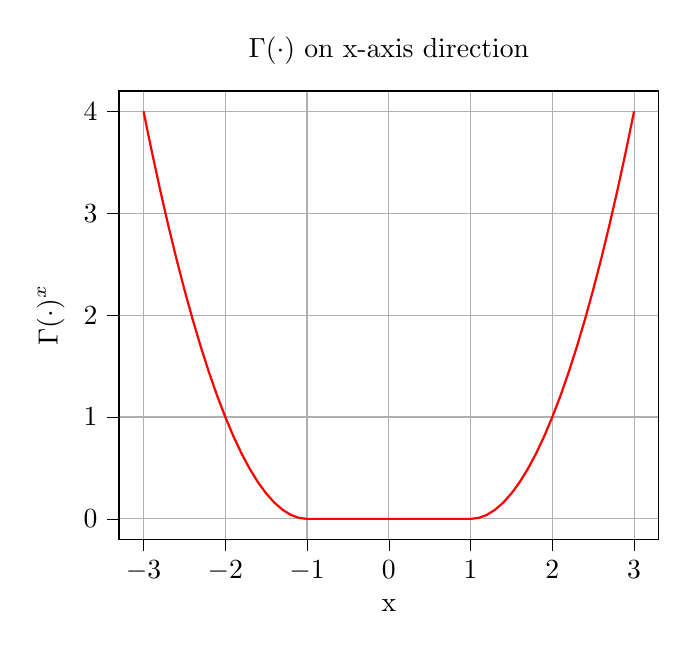
\begin{tikzpicture}

\begin{axis}[
tick align=outside,
tick pos=left,
title={\(\displaystyle \Gamma(\cdot)\) on x-axis direction},
x grid style={white!69.0196078431373!black},
xlabel={x},
xmajorgrids,
xmin=-3.3, xmax=3.30000000000001,
xtick style={color=black},
y grid style={white!69.0196078431373!black},
ylabel={\(\displaystyle \Gamma(\cdot)^x\)},
ymajorgrids,
ymin=-0.200000000000001, ymax=4.20000000000002,
ytick style={color=black}
]
\addplot [thick, red]
table {%
-3 4
-2.9 3.61
-2.8 3.24
-2.7 2.89
-2.6 2.56
-2.5 2.25
-2.4 1.96
-2.3 1.69
-2.2 1.44
-2.1 1.21
-2 0.999999999999998
-1.9 0.809999999999998
-1.8 0.639999999999998
-1.7 0.489999999999998
-1.6 0.359999999999998
-1.5 0.249999999999999
-1.4 0.159999999999999
-1.3 0.0899999999999991
-1.2 0.0399999999999994
-1.1 0.00999999999999966
-0.999999999999998 0
-0.899999999999998 0
-0.799999999999998 0
-0.699999999999998 0
-0.599999999999998 0
-0.499999999999998 0
-0.399999999999998 0
-0.299999999999998 0
-0.199999999999998 0
-0.0999999999999974 0
2.66453525910038e-15 0
0.100000000000003 0
0.200000000000003 0
0.300000000000003 0
0.400000000000003 0
0.500000000000003 0
0.600000000000003 0
0.700000000000003 0
0.800000000000003 0
0.900000000000003 0
1 1.26217744835362e-29
1.1 0.0100000000000006
1.2 0.0400000000000015
1.3 0.0900000000000026
1.4 0.160000000000003
1.5 0.250000000000004
1.6 0.360000000000005
1.7 0.490000000000006
1.8 0.640000000000007
1.9 0.810000000000007
2 1.00000000000001
2.1 1.21000000000001
2.2 1.44000000000001
2.3 1.69000000000001
2.4 1.96000000000001
2.50000000000001 2.25000000000002
2.6 2.56000000000002
2.7 2.89000000000002
2.80000000000001 3.24000000000002
2.90000000000001 3.61000000000002
3.00000000000001 4.00000000000002
};
\end{axis}

\end{tikzpicture}
}}\hfill
  % \subfloat[]{\includegraphics[width=0.475\columnwidth]{clock_penalty.pdf}}
  \includegraphics[width=0.6\columnwidth]{figs/clock_penalty.pdf}
  \caption{The Visualization of clock penalty function $\varGamma_i(\cdot)$ for a single instance.}
  \label{fig:clock_penalty}
\end{figure}
% A visualization of the clock penalty term is shown in \figRef{fig:clock_penalty}.
A visual representation of the clock penalty term can be found in \figRef{fig:clock_penalty}.
% The $\varGamma(\boldsymbol{x}, \boldsymbol{y})$ in \eqRef{eq:opt_relax} is the summation of the clock penalty of all instances, i.e., $\varGamma(\boldsymbol{x}, \boldsymbol{y})=\sum_{i \in \mathcal{V}}\varGamma_i(x_i, y_i)$.
$\varGamma(\boldsymbol{x}, \boldsymbol{y})$ in \eqRef{eq:opt_relax} indicates that the sum of the clock penalty of all instances,
i.e., $\varGamma(\boldsymbol{x}, \boldsymbol{y})$ is equal to $\sum_{i \in \mathcal{V}}\varGamma_i(x_i, y_i)$.
%$\varGamma_i$ is a differentiable, non-negative and convex function, which works well with the rest of the framework.

% The clock penalty multiplier $\eta$ is initialized to 0.
Initially, the clock penalty multiplier $\eta$ is set to a value of 0.
% Each time we reset the clock penalty function $\varGamma(\cdot)$,
% we update $\eta$ with the relative ratio between the gradient norms of the wirelength and the clock penalty to maintain stability,
As soon as we reset the clock penalty function $\varGamma(\cdot)$,
we update $\eta$ with the relative ratio between the gradient norms of the wirelength and the clock penalty in order to maintain the stability of the clock penalty function.
\begin{equation}
  \eta = \frac{\iota \norm{\nabla \widetilde{\mathcal{T}}_{\omega}}_1}{\norm{\nabla \varGamma}_1+ \varepsilon}.
\end{equation}
% We observe that only 1\% of instances are out of their available clock regions right after the clock region assignment, so most instances have zero penalties.
As we observe, only 1\% of the instances are out of their available clock regions right after they have been assigned the clock region, so most instances have no penalties as a result of this.
% To balance the gradient norm ratio, $\iota$ is empirically set to $10^{-4}$, and $\varepsilon$ is set to
% $10^{-2}$ to avoid numerical explosion.
It is empirically established that $\iota$ is equal to $10^{-4}$ and $\varepsilon$ is equal to $10^{-2}$ as a method of balancing the gradient norm ratio.




\iffalse
\textcolor{blue}{
\subsection{Area Inflation-based Routability Optimization}
\label{sec:route_opt}
Under our electrostatic formulation, we adopt the area inflation-based technique to resolve routing congestion \cite{PLACE_TCAD2021_Meng}.
At the beginning of the placement, instances are set to their original areas.
Each time the inner sub-optimization problem $\mathcal{L}_2$ \eqRef{eq:nested_opt_area} converges, we inflate the instances according to their location's routing congestion estimation and pin density.
This indicates that instances in routing congested areas will gain a larger inflation ratio,
which analogously means that they will have a higher amount of charges in the electrostatic system (see \figRef{fig:electrostatics_analogy}).
In this way, instances will be spread out from the routing congested areas.
}

\subsection{Clock-Aware Legalization \& Detailed Placement}
\label{sec:ca_legal_cp}

%In this section, we introduce our clock-aware legalization and detailed placement algorithms.
We adapt the algorithms in \cite{PLACE_TCAD2019_Li_UTPLACEF_DL} to handle LUT, FF, distributed RAM, and SHIFT for clock-aware legalization.
We also design a clock-aware multistage independent set matching (ISM) algorithm for detailed placement like that in \cite{PLACE_TCAD2019_Li_UTPLACEF_DL}.
Due to the page limit, we omit the details.
\fi

\iffalse
\subsubsection{Clock-Region-wise Direct Legalization}

Since FPGA contains heterogeneous resources, the legalization for each type of resource happens at different stages in the flow.
DSPs and BRAMs are legalized when the overflow is less than 15\% during global placement.
We fix their locations and continue global placement iterations until the overflow is lower than 10\%.
Then we finish global placement and legalize the rest of the instances.

DSP, BRAM, and CARRY are legalized with a min-cost  flow-based assignment method to minimize displacement. Clock legality is ensured by removing the edges between instances and clock-illegal sites from the assignment graph.
We adopt the two-phase direct legalization algorithm in \cite{PLACE_TCAD2019_Li_UTPLACEF_DL} for the legalization of LUT, FF, distributed RAM, and SHIFT.
Whether a SLICEM is configured as LUT or distributed RAM or SHIFT is greedily determined in the first phase by the type of the first instance placed.
Clock region constraints are satisfied in the second phase, where instances in illegal clock regions are ripped up to search for legal locations.
%To account for SLICEL-SLICEM heterogeneity, a SLICEM's mode is dynamically determined when the first LUT/SHIFT/distributed RAM is placed there.

\subsubsection{Scoreboard-based Half-column Legalization}
\label{sec:hc_lg}
As referenced in \secRef{sec:clock_constraint}
, in addition to clock region constraints, instances in each half column must not use more than 12 clock nets.
%Since this is a quite loose requirement (each clock region has 30 half columns, so with the clock region constraint of 24 clock nets, the half column constraint would be broken only with extreme imbalance of distribution), this constraint is ignored in global placement.
An iterative process similar to the generation of clock region assignments is developed.
We keep a \emph{scoreboard} to record which clock nets are allowed in each half-column region, as well as a cost for each clock net's presence in each half-column region.
Initially, all clock nets are allowed in all regions.
After legalization, if the half-column constraint is not satisfied, then the clock with the highest cost is prohibited in those half-columns with more than 12 clock nets.
The next iteration of legalization is performed with these prohibitions.
The process continues until a half-column-legal solution is reached.

\subsubsection{Detailed Placement}

A multi-stage independent set matching algorithm is used for detailed placement. We maintain clock legality by ignoring swaps that would break the constraints.

\fi


\subsection{Timing-Criticality-based Weighting Method}
\label{sec:timing_opt}

\begin{figure*}[tb]
   \centering
   \includegraphics[width=\textwidth]{figs/timing_analysis.pdf}
   \caption{
     An illustration for the static timing analysis on FPGA. Support the clock period is $T$ and the signal arrival time at primary input ports has minor skew.
     The required arrival time at the sink of a timing path is the clock period minus the clock delay at the capture FFs and the setup time of FFs (1ps in our example),
     and the required arrival time of a timing endpoint is determined by the required arrival time of its fanout endpoints and the fanout edge delays.
     The actual arrival time of a timing endpoint is the maximal accumulated delay from the primary inputs.
     The slack of a timing edge is the difference between the required arrival time at its sink, and the summation of the actual arrival time at its source and its edge delay.
    }
   \label{fig:timing_analysis}
   \vspace{-.2in}
\end{figure*}

The timing performance objective $\widetilde{\mathcal{T}}_{\boldsymbol{\omega}}(\cdot)$ (see \eqRef{eq:opt_relax}) consists of two components:
i) the wirelength objective as a first-order approximation of WNS and TNS, and ii) the net criticality $\boldsymbol{\omega}$ that remedies the lack of timing information for first-order approximation.
\begin{equation}
  \widetilde{\mathcal{T}}_{\boldsymbol{\omega}}(\boldsymbol{x}, \boldsymbol{y}) = \sum\limits_{e \in E} \omega_e \cdot \widetilde{W}(e)
\end{equation}
$\omega_e \in \boldsymbol{\omega}$ measures the timing criticality of nets, i.e., 
whether any timing path through nets violates timing constraints, 
what is the degree of the violation, 
and how much the path delay can be reduced.
%
In this section we detail how $\widetilde{\mathcal{T}}(\cdot)$ functions.

\subsubsection{Static Timing Analysis}
\label{sec:static_timing_analysis}
%
Timing-driven placement leverages the static timing analysis (STA) to evaluate
the timing criticality of nets.
%
STA relies on (i) model of signal delays for nets and instances, and (ii) a timing analysis engine based on net and instance delays.
%

Delay models in FPGA are highly coupled with the pre-fabricated routing architecture and the behavior of the FPGA router.
%
In our experiment, we design the linear delay model, where the delay of the routing path between a source endpoint and a sink endpoint is calculated
by the Manhattan distance between them. 
% \textcolor{red}{
% (Jing) The delay model in placement is, we assume the routing path from a source endpoint to a sink endpoint follows the Manhattan distance.
% We have litter contribution on this, and I suppose it can be described simply.
% }
Given the delay of the timing edges, the timing analysis engine determines which timing paths violate their timing constraints.
A timing path $\pi$ is a directed acyclic path for particular source and sink pairs (primary I/Os and I/Os of store elements).
The delay $t_\pi$ along a path $\pi$ is the sum of wire delays and cell delays,
and every path comes with a timing constraint $c_\pi$ defined via the \textit{actual arrival time (AAT)} and \textit{required arrival time (RAT)} for every driver pin and primary output.

The slack $s_\pi$ of a path $\pi$ is defined as $s_\pi = c_\pi - t_\pi$.
We mainly focus on the \textit{setup time} constraint, which is defined as the difference between the AAT and RAT.
A timing path $\pi$ violates the setup time constraints if the slack is negative.
The slack of a timing edge is the smallest path slack among the paths containing this edge.
To avoid enumerating all paths, we compute the slack from the actual arrival times and required arrival times at timing endpoints \cite{OpenTimer_ICCAD2015_Huang}.
\begin{subequations}
  \label{eq:att_rat}
  \begin{align}
    T_{ATT}(v_i) &= \max_{v_j \in fanin(v_i)} T_{ATT}(v_j) + e_{j,i} \\
    T_{ATT}(v_i) &= \min_{v_j \in fanout(v_i)} T_{RAT}(v_j) - e_{i,j}
  \end{align}
\end{subequations}
In \eqRef{eq:att_rat}, $v_i$ is an endpoint in the timing graph, and $e_{i,j}$ denotes the timing delays from endpoint $i$ to endpoint $j$, provided by the delay model.
The slack of timing edge $s_{i,j}$ connecting the source endpoint $v_i$ and the sink endpoint $v_j$ is
\begin{equation}
  s_{i,j} = T_{RAT}(v_j) - T_{ATT}(v_i) - e_{i,j},
\end{equation}
\figRef{fig:timing_analysis} illustrates the timing analysis process.


\subsubsection{Timing-driven Net Reweighting Scheme}
In the timing graph, nets have diverse effects on the timing slacks.
Those nets with higher timing criticality should be more sensitive to the timing closure.
To improve the timing in the analytical placement framework, we assign different net weights to different nets based on their timing criticality.
Let $s_e$ and $s_{wns}$ denote the timing slacks of net $e$ and the worst negative slack, respectively.
% $s_e$ is empirically denoted as the minimal timing edge slacks between its source and sink pairs.
We define the timing criticality $c_e$ as follows,

\begin{equation}
  \label{eq:timing_crit}
  c_e = \frac{\min(0, s_e)}{\min(0, s_{wns})-T} \in [0, 1),
\end{equation}
%
where $T$ is the clock period.
%
% When there are no timing violating path passing through net $e$, i.e., $s_e \geq 0$,
When net $e$ is not on a path with timing violation, i.e. $s_e \geq 0$, the
timing criticality $c_e$ remains zero. Otherwise, the timing criticality equals the ratio $\frac{\vert s_e \vert}{\vert s_{wns} \vert+T}$.
%
The worse timing slack $\vert s_e \vert$ is, the larger timing criticality $c_e$ it will have.
The largest timing criticality falls upon the nets on the most critical path.

After evaluating the timing criticality, we compute the net weight $w_e \in \boldsymbol{\omega}$ as
\begin{subequations}
  \label{eq:timing_weight}
  \begin{align}
    \beta_e &= \alpha \cdot \max\left(1, \exp(c_e)\right) \\
    \omega_e' &\leftarrow \omega_e \cdot \beta_e \
  \end{align}
\end{subequations}
where $\omega_e'$ is the updated net weight, $\beta_e$ denotes the reweighting magnitude for net $e$, and $\alpha$ is a hyper-parameter that controls the weighting magnitude
\footnote{
In our experiments, $\alpha$ equals 1.
}.

\iffalse
\begin{figure}[tb]
   \centering
   \includegraphics[width=\columnwidth]{figs/timing_curve.pdf}
   \caption{
    Relationship between the reweighting magnitude $\beta_e$ and the clock period $T$ for paths with different timing slacks.
    $T_{target}$ denotes the target clock period. The outermost blue curve represents the most critical path $\beta_{wns}$ with maximal delay $T_{max}$.
    Other curves represent the paths with different timing slacks, and $\Delta$ denotes their delay difference with the worst path $\omega_{wns}$.
    }
   \label{fig:timing_curve}
   \vspace{-.2in}
\end{figure}
\fi

\definecolor{tradewind}{HTML}{64B5AC}

\begin{figure}[tb]
    \centering
    \subfloat[]{\includegraphics[width=\columnwidth]{figs/timing_w-t.pdf}\label{fig:timing_w-t}} \hfill
    \subfloat[]{\includegraphics[width=\columnwidth]{figs/timing_w-d.pdf}\label{fig:timing_w-d}}
    \caption{
        %
      (a) This figure illustrates the relationship between the reweighting
      magnitude $\beta_e$ and the clock period $T$ given a certain path and its
      delay.
      %
    In particular, the path with delay $d_{wns}$ represents the most critical
    path.
    %
    This figure also depicts another path with delay $d_{wns}-\Delta$, where
    $\Delta$ measures how much the delay is smaller the worst-case path
    $d_{wns}$.
    %
    (b) This figure shows the relationship between the reweighting magnitude
    $\beta_e$ and the path delay $d_e$ given a clock period.
    %
    This figure plots two curves for two certain clock periods
    $T_1$ and $T_2$ ($T_2 < T_1 < d_{wns}$).
    %
    % Under both scenarios, there always exists paths whose delay exceeds
    % the period. 
    % Nevertheless, the reweighting magnitude only makes an effect on those paths
    % whose delay violates constraints no matter what the clock period is. 
    }
\end{figure}

\subsubsection{Effectiveness Analysis of the Rweighting Scheme}
\label{sec:tdp_effectiveness_analysis}
It is suggested that our reweighting scheme can control the reweighting scale according to the severity of the target timing constraints.
The reweighting magnitude $\beta_e$ of a net is determined by the largest magnitude of the timing paths that pass through it,
i.e., $\beta_e = \max\limits_{\pi \ni e} \beta_{\pi}$.
We then gave a brief analysis of how the timing path $\pi$ affects the re-weighting scheme in nets.

%
For the paths with maximal delay $d_{wns}$, the intuition is that the reweighting method should make no effect, i.e., $\beta_{wns}$ equals 1, when
it has no timing violations.
%
Otherwise, the smaller $T-d_{wns}$ is, the larger the reweighting magnitude
should be.
%
\figRef{fig:timing_w-t} show the relationship between the magnitude of the reweighting $\beta_{wns}$ and the clock period $T$ for a certain path and its delay. 
%
This figure demonstrates that a path will only gain a reweighting magnitude greater than one when the target clock period $T$ is less than its path delay.
%
The reweighting magnitude will grow faster with $T$ becoming smaller. 
%
\figRef{fig:timing_w-d} regards the path delay as a variable and shows how
the reweighting magnitude $\beta_{wns}$ reacts under a certain clock period.
%
The relationship curves align with our intuition that nets with a smaller timing delay
always gain a smaller reweighting magnitude.
%
No matter what the clock period is, the reweighting magnitude only takes effect
on those paths with timing violations. 
%
% To avoid numerical explosion, we can also control the magnitude range through the parameter $\alpha$.

% We omit the derivation detail for the sake of brevity.
Nets on critical paths gain a larger weighting magnitude in this stage.
In the subsequent analytical placement step, the increased net weights
then help critical paths tilt more toward timing closure in the tradeoff
between timing and area.
